\begin{frame}{Laser Power}
	The laser has a power of:
	$$P(t) \propto e^{-(t-t_0)^ / 2\sigma^2}$$
	with a total energy:
	\begin{align*}
		E = \int S(t) dt = P_\text{Average} / f \approx \SI{1.2}{W} / \SI{100}{MHz} = \SI{12}{uJ}
	\end{align*}
\end{frame}

\begin{frame}{Absorption}
	only a fraction $A=1$ is absorbed into a volume given by the laser radius $r\approx \SI{200}{um}$ and the optical depth $d\approx \SI{250}{nm}$:
	$$V=\pi r^2 \cdot d$$
	$$S = \frac{P}{V}\; A$$
	with $[S] = W/m^3$  
\end{frame}

\begin{frame}{e$^-$ Gas}
	The temperature change due to absorption can be calculated with the molar Volume $V_m = M / \rho$ and  the specific heat capacity $c_e= 1/M \; dQ/dT$.\\
	The lattice relaxation time $g\approx\SI{300}{fs}$. \customcite{stange_hot_2015}\\
	Diffusion is neglected.
	Radiative cooling is also ignored.
	\begin{align*}
		\frac{dT_e}{dt}
		&= \frac{V_m}{c_e(T)}S\\
		&- \frac{T_e - T_l}{g}\\ 
		&\textcolor{seegrau}{- \frac{T_e - T_\text{Room}}{\tau_e}}
	\end{align*}
\end{frame}

\begin{frame}{Lattice Temperature}
	For now the lattice temperature is assumed to be constant.
	\textcolor{seegrau}{
		For the lattice it is similar with the diffusion $\tau_l\approx$:
		\begin{align*}
			\frac{dT_l}{dt}
			&= \frac{T_e - T_l}{g}\\ 
			&- \frac{T_e - T_\text{Room}}{\tau_l}
		\end{align*}
	}
\end{frame}

\begin{frame}
	\centering
	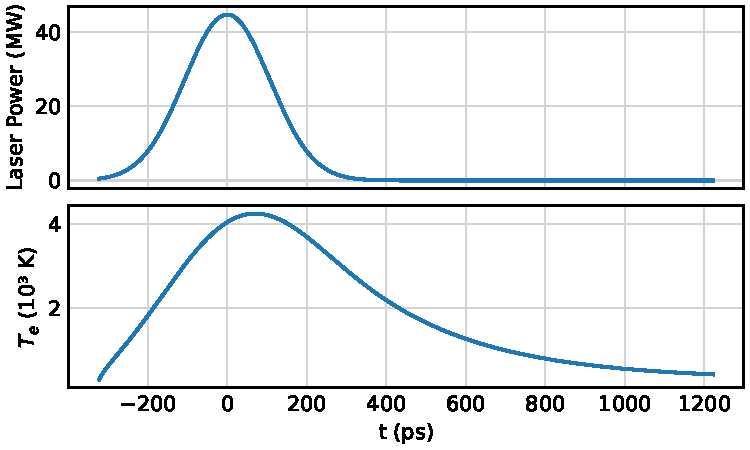
\includegraphics[width=.8\textwidth]{../model/figures/temperature profile.pdf}
\end{frame}

\begin{frame}
	\begin{columns}
		\column{.5\textwidth}
		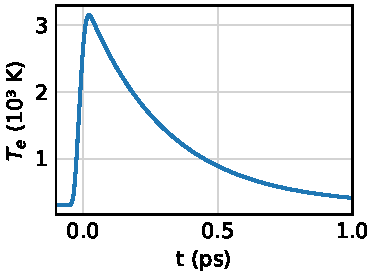
\includegraphics[width=\textwidth]{../model/figures/temperature stange_hot_2015.pdf}

		\column{.5\textwidth}
		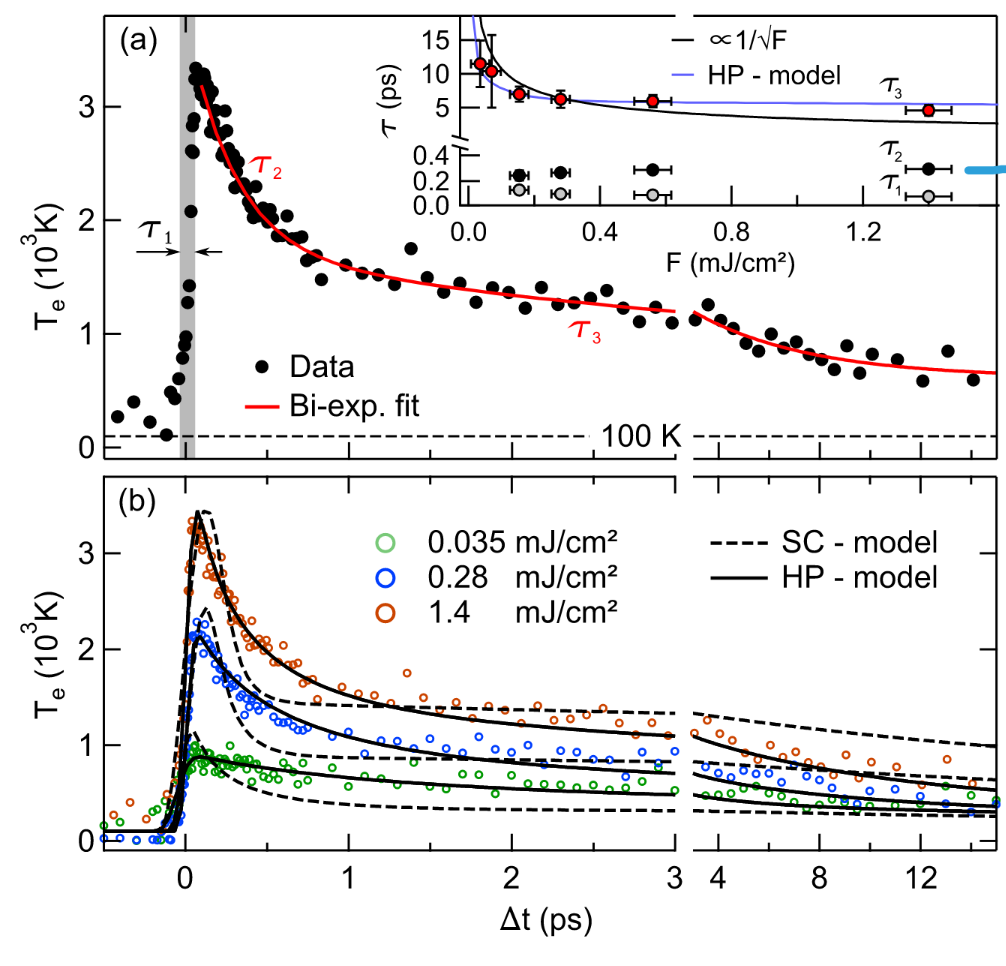
\includegraphics[width=\textwidth]{./figures/stange_hot_2015.png}
	\end{columns}
	\customcite[Fig. 4]{stange_hot_2015}
\end{frame}

\begin{frame}
	\centering
	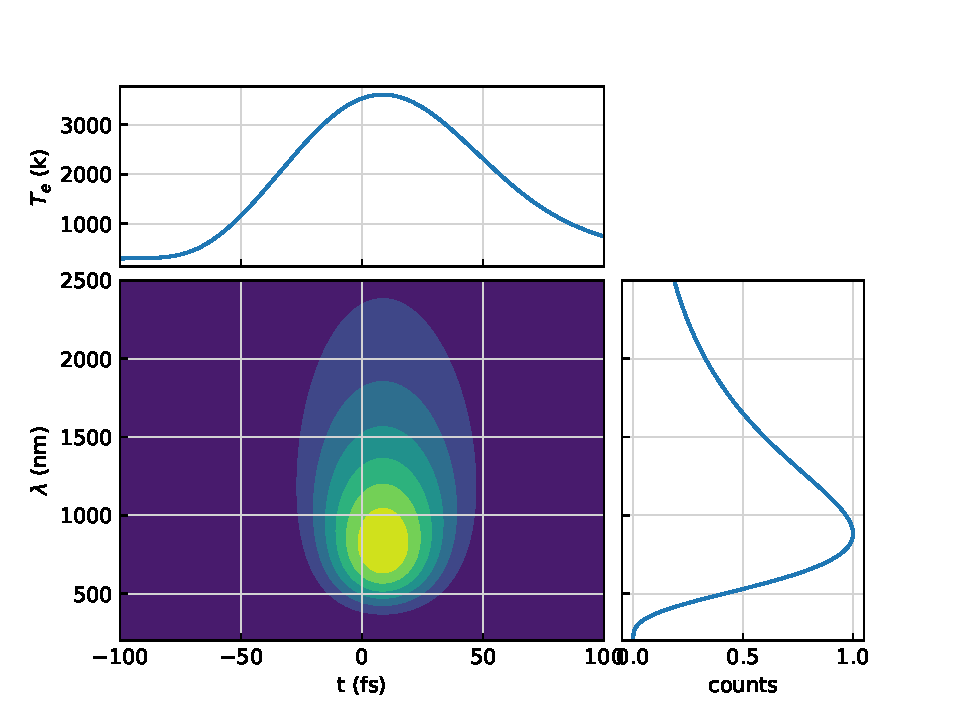
\includegraphics[width=.8\textwidth]{../model/figures/steak view.pdf}
\end{frame}
